% Homework template for Inference and Information
% UPDATE: September 26, 2017 by Xiangxiang
\documentclass[a4paper]{article}
\usepackage{ctex}
\usepackage{amsmath, amssymb, amsthm}
\usepackage{moreenum}
\usepackage{mathtools}
\usepackage{url}
\usepackage{bm}
\usepackage{enumitem}
\usepackage{graphicx}
\usepackage{listings}
\usepackage{color}

\lstset{
    basicstyle          =   \sffamily,          % 基本代码风格
    keywordstyle        =   \bfseries,          % 关键字风格
    commentstyle        =   \rmfamily\itshape,  % 注释的风格,斜体
    stringstyle         =   \ttfamily,  % 字符串风格
    flexiblecolumns,                % 别问为什么,加上这个
    numbers             =   left,   % 行号的位置在左边
    showspaces          =   false,  % 是否显示空格,显示了有点乱,所以不现实了
    numberstyle         =   \zihao{-5}\ttfamily,    % 行号的样式,小五号,tt等宽字体
    showstringspaces    =   false,
    captionpos          =   t,      % 这段代码的名字所呈现的位置,t指的是top上面
    frame               =   lrtb,   % 显示边框
}

\lstdefinestyle{Python}{
    language        =   Python, % 语言选Python
    basicstyle      =   \zihao{-5}\ttfamily,
    numberstyle     =   \zihao{-5}\ttfamily,
    keywordstyle    =   \color{blue},
    keywordstyle    =   [2] \color{teal},
    stringstyle     =   \color{magenta},
    commentstyle    =   \color{red}\ttfamily,
    breaklines      =   true,   % 自动换行,建议不要写太长的行
    columns         =   fixed,  % 如果不加这一句,字间距就不固定,很丑,必须加
    basewidth       =   0.5em,
}
\usepackage{subcaption}
\usepackage{booktabs} % toprule
\usepackage[mathcal]{eucal}
\usepackage[thehwcnt = 2]{iidef}

\thecourseinstitute{清华大学电子工程系}
\thecoursename{\textbf{媒体与认知} \space 课堂2}
\theterm{2021-2022学年春季学期}
\hwname{作业}
\begin{document}
\courseheader{test}
\name{李智毅}
\vspace{3mm}
\centerline{\textbf{\Large{理论部分}}}

\section{单选题(15分)}
\subsection{\underline{D}}

\subsection{\underline{C}}

\subsection{\underline{B}}

\subsection{\underline{C}}

\subsection{\underline{D}}

\section{计算题(15 分)}
\subsection{设隐含层为$\mathbf{z}=\mathbf{x}\mathbf{W}^T+\mathbf{b}$,其中$\mathbf{x}\in R^{(1 \times m)}$,$\mathbf{z}\in R^{(1\times n)}$,$\mathbf{W}\in R^{(n\times m)}$,$\mathbf{b} \in R^{(1\times n)}$均为已知,其激活函数如下:
$$\mathbf{y}=\tanh(\mathbf{z})=\frac{e^\mathbf{z}-e^{-\mathbf{z}}}{e^\mathbf{z}+e^{-\mathbf{z}}}$$
若训练过程中的目标函数为L,且已知L对$\mathbf{y}$的导数 $\frac{\partial L}{\partial \mathbf{y}}=[\frac{\partial L}{\partial y_1},\frac{\partial L}{\partial y_2},...,\frac{\partial L}{\partial y_n}]$和$\mathbf{y}=[y_1,y_2,...,y_n]$的值。}
\subsubsection{请使用$\mathbf{y}$表示出$\frac{\partial \mathbf{y}}{\partial \mathbf{z}}$}
\begin{equation}
    \frac{\partial \mathbf{y}}{\partial \mathbf{z}} = \frac{(e^{\mathbf{z}} + e^{\mathbf{z}})^2 - (e^{\mathbf{z}} - e^{\mathbf{z}})^2}{(e^{\mathbf{z}} + e^{\mathbf{z}})^2} = \mathbf{1} - \mathbf{y}^2
\end{equation}
其中,$ \mathbf{1} $ 指$ (1 \times N) $维全为$ 1 $的向量;$ \mathbf{y}^2 $指向量$ \mathbf{y} $之间逐元素求平方。

\subsubsection{请使用$\mathbf{y}$和$\frac{\partial L}{\partial \mathbf{y}}$表示$\frac{\partial L}{\partial \mathbf{x}}$,$\frac{\partial L}{\partial \mathbf{W}}$,$\frac{\partial L}{\partial \mathbf{b}}$。}
提示:$\frac{\partial L}{\partial \mathbf{x}}$,$\frac{\partial L}{\partial \mathbf{W}}$,$\frac{\partial L}{\partial \mathbf{b}}$与x,W,b具有相同维度。
\begin{equation}
\begin{aligned}
    \frac{\partial L}{\partial \mathbf{x}} &= \left[\sum_{j=1}^N \frac{\partial L}{\partial z_j} \frac{\partial z_j}{\partial x_1}, \sum_{j=1}^N \frac{\partial L}{\partial z_j} \frac{\partial z_j}{\partial x_2}, ..., \sum_{j=1}^N \frac{\partial L}{\partial z_j} \frac{\partial z_j}{\partial x_m}\right] \\
    &= \left(\frac{\partial L}{\partial \mathbf{y}} * (\mathbf{1} - \mathbf{y}^2)\right) \mathbf{W}
\end{aligned}
\end{equation}
\begin{equation}
    \frac{\partial L}{\partial W_{ij}} = \sum_{k=1}^N \frac{\partial L}{\partial z_k} \frac{\partial z_k}{\partial W_{ij}} = x_j \frac{\partial L}{\partial z_i}
\end{equation}
\begin{equation}
    \frac{\partial L}{\partial \mathbf{W}} = \frac{\partial L}{\partial \mathbf{z}} \mathbf{x} = \left(\frac{\partial L}{\partial \mathbf{y}} * (\mathbf{1} - \mathbf{y}^2)\right) \mathbf{x}
\end{equation}
\begin{equation}
    \frac{\partial L}{\partial \mathbf{b}} = \frac{\partial L}{\partial \mathbf{z}} = \frac{\partial L}{\partial \mathbf{y}} * (\mathbf{1} - \mathbf{y}^2)
\end{equation}
其中"*"为逐元素相乘。

\vspace{6mm}
\centerline{\textbf{\Large{编程部分}}}
\vspace{3mm}
% 请根据是否选择自选课题的情况选择“编程作业报告”或“自选课题开题报告”中的一项完成
\section{编程作业报告}
\subsection{完成线性分类器的程序代码}
\subsubsection{losses.py}
按照要求计算修正的softmax函数,将label转化为onehot编码;\\
按照定义计算交叉熵,返回loss(具体见代码)
\subsubsection{network.py}
按照定义计算线性层的前向传播函数,保存数据至ctx;\\
计算反向传播函数,通过grad\_output计算grad\_W, grad\_b及grad\_input;\\
使用nn.Parameter()初始化W、b为可训练的参数;\\
将相应的线性层加入模型中(具体见代码)
\subsubsection{recognition.py}
按照需要实例化MLP模型及损失函数;\\
完成训练过程及反向传播、参数更新;\\
读取模型(具体见代码)
\subsection{训练、测试、可视化}
\subsubsection{训练}
\textbf{使用默认参数训练}\\
训练过程:(图1)\\
\begin{figure}
    \centering
    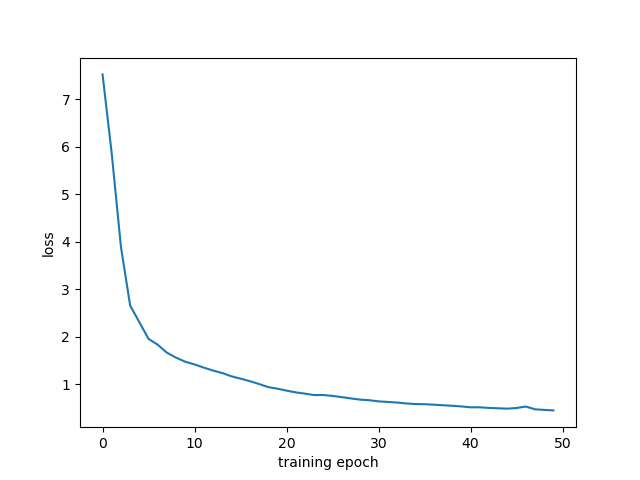
\includegraphics[width=12cm]{Fig1.png}
    \caption{默认参数训练loss}
\end{figure}
测试过程:(图2)\\
\begin{figure}
    \centering
    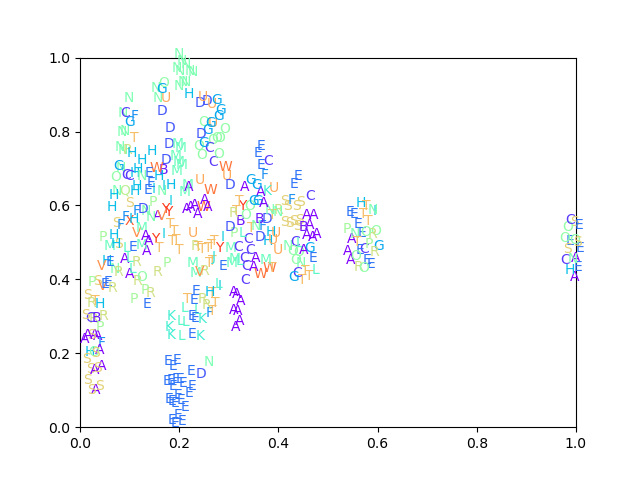
\includegraphics[width=12cm]{Fig2.png}
    \caption{默认参数测试可视化}
\end{figure}
测试结果准确率为67.8\%

\textbf{采用Adam优化器训练}\\
训练过程:(图3)\\
\begin{figure}
    \centering
    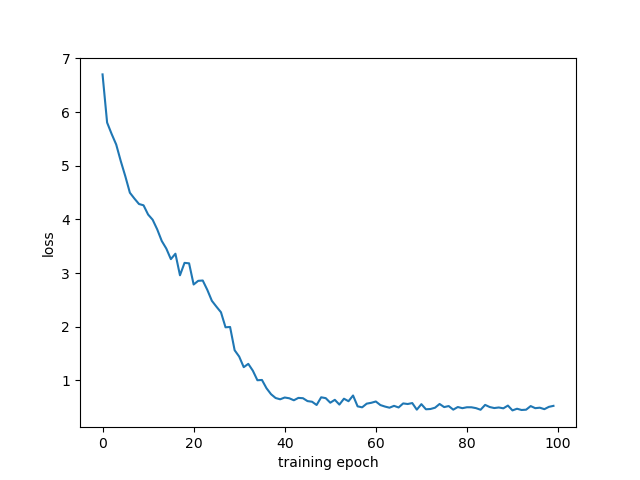
\includegraphics[width=12cm]{Fig3.png}
    \caption{Adam优化器训练loss}
\end{figure}
测试过程:(图4)\\
\begin{figure}
    \centering
    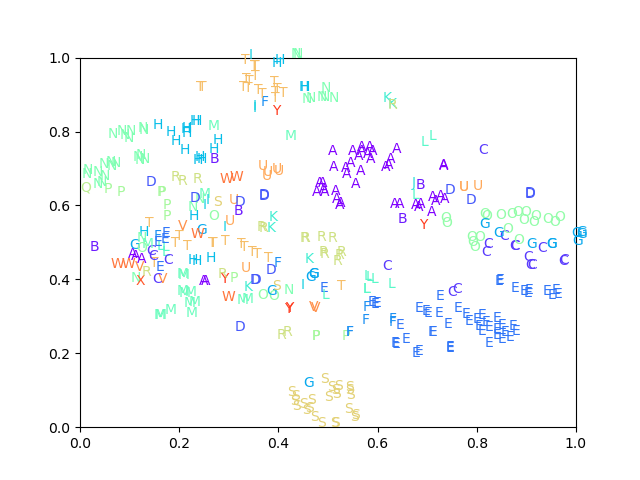
\includegraphics[width=12cm]{Fig4.png}
    \caption{Adam优化器测试可视化}
\end{figure}
测试结果准确率为77.8\%,优于默认参数

\subsubsection{可视化}
比较好的可视化图见图4,将不同字母相对分开

\subsubsection{预测图像类别}
预测predict01(图5)的结果为A\\
\begin{figure}
    \centering
    \includegraphics[width=2cm]{../data/character_classification/new_images/predict01.png}
    \caption{predict01图像}
\end{figure}
预测predict02(图6)的结果为B\\
\begin{figure}
    \centering
    \includegraphics[width=2cm]{../data/character_classification/new_images/predict02.png}
    \caption{predict02图像}
\end{figure}

\textbf{代码见附件}

\end{document}



%%% Local Variables:
%%% mode: late\rvx
%%% TeX-master: t
%%% End:
